\documentclass{beamer}

\usetheme{Madrid}

\usepackage{graphicx} % Allows including images
\graphicspath{{./../img/}}

\title{Theia Primer}

\author{Optics Group, Virgo}
\date{Wednesday, May 10\textsuperscript{th} 2017} % Date, can be changed to a custom date

\begin{document}

\begin{frame}
\titlepage % Print the title page as the first slide
\end{frame}




%------------------------------------------------

\begin{frame}
\frametitle{Modeling Gaussian beams}
\begin{itemize}
\item General astigmatic Gaussian beam in an orthogonal basis $(k, e_1, e_2)$:

$$ E(\vec r, t) = \mathrm{exp}[ i \eta(z) -i\frac{k}{2} {}^t (x,y) Q(z) (x,y)] e^{i(\omega t - kz)} $$

\item $(x,y)$ is the transversal coordinate in the $(e_1, e_2)$ basis, $Q$ is a symmetrical tensor:

\[ \left( \begin{array}{cc}
\frac{\cos^2 \theta}{q_x(z)} + \frac{\sin^2 \theta}{q_y(z)} & \frac{1}{2} \sin2\theta \left(\frac{1}{q_x(z)}  - \frac{1}{q_y(z)}\right)\\
\frac{1}{2} \sin2\theta \left(\frac{1}{q_x(z)}  - \frac{1}{q_y(z)} \right) & \frac{\sin^2 \theta}{q_x(z)} + \frac{\cos^2 \theta}{q_y(z)} \end{array} \right)\] 

\item Specification parameters: $\theta, q_{x,y} \in \mathbb{C}$, $(e_1, e_2)$ basis.

\item \textbf{Approximations:} ROC(beam) $ \gg $ ROC(surface) (+ paraxial)

\item Geometric optics: no approximation
\end{itemize}
\end{frame}

\begin{frame}
\frametitle{What can it do?}

\begin{table}
\begin{center}
\begin{tabular}{p{3.5cm} | p{3.5cm}| p{3.5cm}}
\textbf{Yes} & \textbf{No} & \textbf{Not yet} \\ \hline
Non-sequential propagation & Higher order modes & Cavities \\
Sequential propagation & Beam saving & Interferences \\
General astigmatic beams & Surface action specification & Export to CAD software\\
 & Grating surfaces &  \\
 & (Polarization) & \\
\end{tabular}
\end{center}
\end{table}
\end{frame}


\begin{frame}
\frametitle{Data structures/algorithm/approximations}
\begin{center}
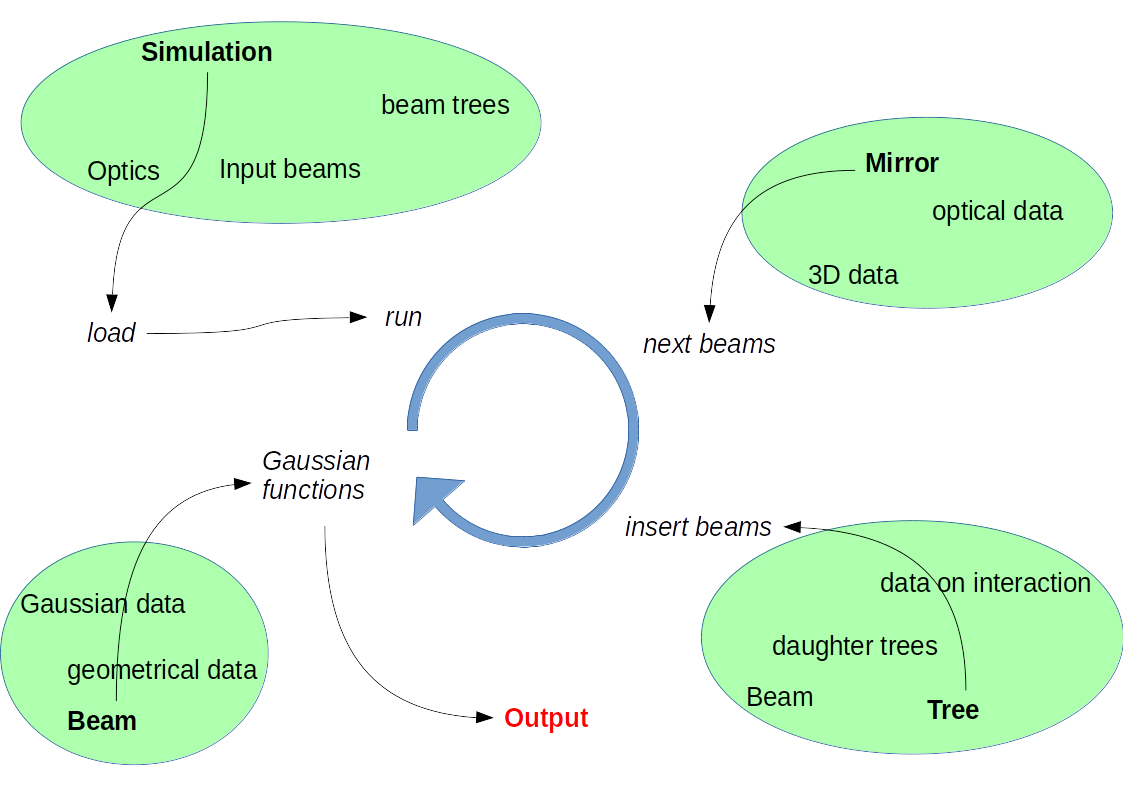
\includegraphics[scale=0.35]{flow}
\end{center}

\end{frame}

%------------------------------------------------

\begin{frame}
\frametitle{Demonstration}
\begin{itemize}
\item Comparison with \texttt{OptoCAD} for 2D tracing (\texttt{telescope.py})
\item An example in 3D with spherical mirrors (\texttt{sphere.py})
\end{itemize}
\end{frame}


\begin{frame}
\frametitle{Benchmarking: time (i7/8GB)}

\begin{center}
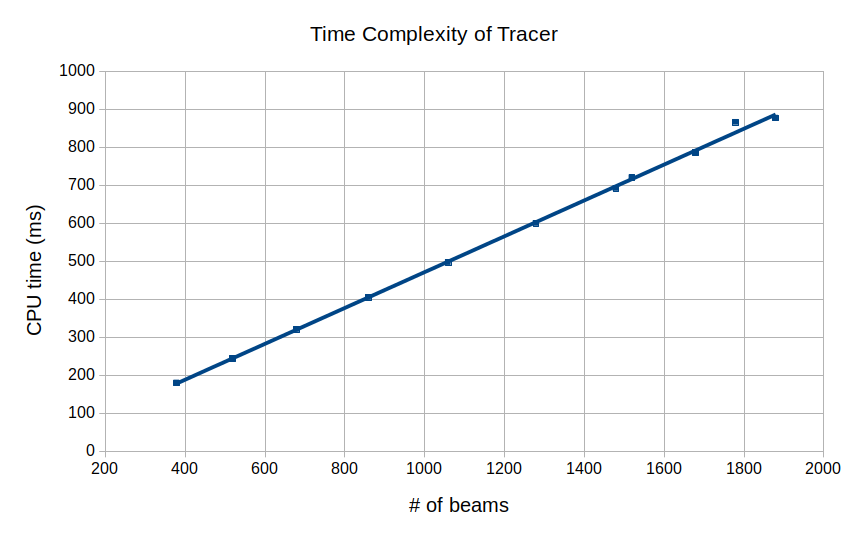
\includegraphics[scale = .45]{timecomplexity.png}
\end{center}


\begin{itemize}
\item CPU = 0.47ms $\times$ (\# beams) ($R^2 = 99.95$\%)
\end{itemize}

\end{frame}

\begin{frame}
\frametitle{Benchmarking: space (i7/8GB)}

\begin{center}
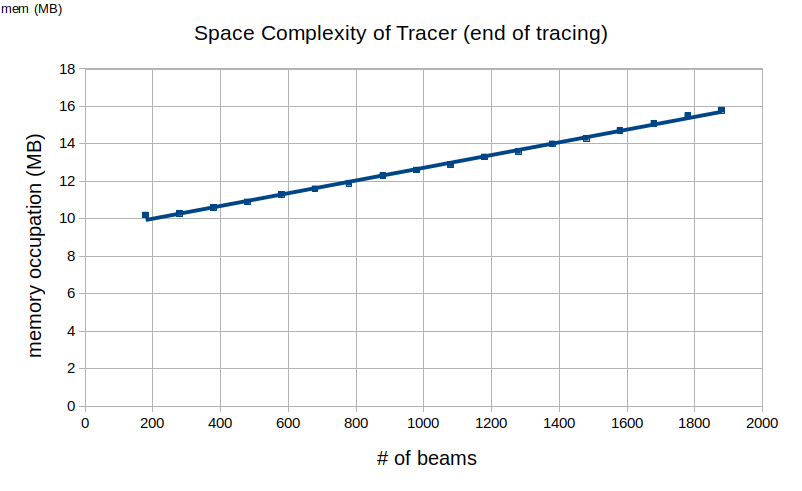
\includegraphics[scale = .45]{spacecomplexity.png}
\end{center}


\begin{itemize}
\item Mem. = 9,3MB + 3,4kB/beam ($R^2 = 99.76$\%)
\end{itemize}
\end{frame}

\begin{frame}
\frametitle{Next steps}
\begin{figure}
\begin{center}
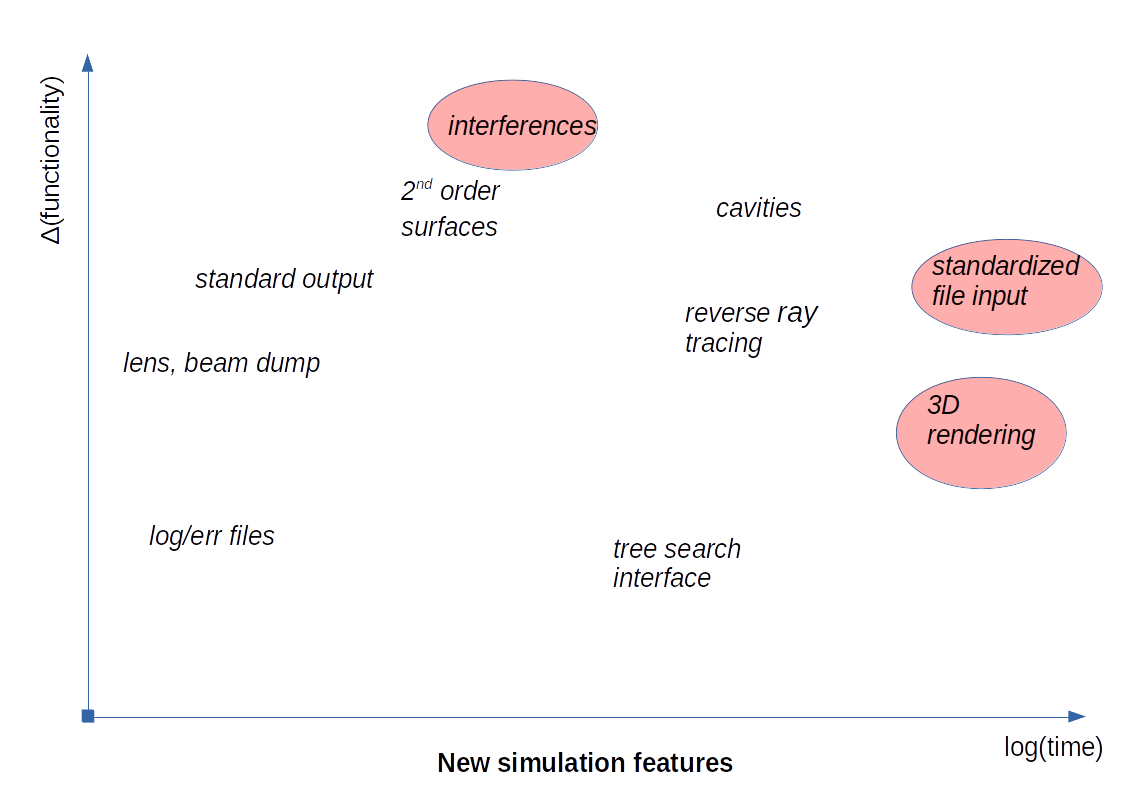
\includegraphics[scale=0.36]{newfeatures}

\end{center}
\end{figure}
\end{frame}


\begin{frame}

\frametitle{References}

\begin{thebibliography}{99} 

\bibitem{1}
Kochkina, Wanner, Schmelzer, Tr\"obs, Heinzel:
\textit{Modeling of the General Astigmatic Gaussian Beam and its Propagation through 3D Optical Systems},
Applied Optics 24 (2013)

\bibitem{2}
Arnaud, Kogelnik:
\textit{Gaussian Light Beams with General Astigmatism},
Applied Optics 8 (1969)

\end{thebibliography}

\end{frame}


\end{document} 
